\chapter{Recuperación de imágenes basadas en su contenido (CBIR)}

En el contexto de las ciencias de información, en el Capítulo 1 de \cite{10.5555/1394399} podemos encontrar una definición genérica para el contexto de las ciencias de computación del término "recuperación de información" que dice que:

\begin{definicion}
La recuperación de información, o \emph{information retrieval (IR)}, consiste en encontrar material de una naturaleza no estructurada que satisface una necesidad de información dentro de grandes colecciones.
\end{definicion}

En particular, nos encontramos trabajando en la recuperación de imágenes que pertenece a la categoría de recuperación de información multimedia. Este, a su vez, se divide en dos tipos de recuperación, las basadas en texto, \emph{text-based image retrieval (TBIR)}, o las basadas en su contenido, \emph{content-based image retrieval (CBIR)}.\\

En \cite{content-based} se dice, en que los sistemas TBIR, los usuarios utilizan palabras clave o descripciones de las imágenes como consulta en una base de datos para recuperar las imágenes que sean relevantes a la palabra clave. Para ello, primeramente las imágenes deben de ser anotados con texto ya sea de forma manual o automática. Esto posee la desventaja de que los algoritmos de anotación automática de imágenes no son factibles para generar textos descriptivos para un amplio espectro de imágenes requiriendo la anotación manual que, a su vez, suele ser subjetiva y dependiente del contexto. Como ventaja, al realizar utilizar únicamente texto para describir la imagen, sus consultas son rápidas ya que la coincidencia de cadenas es un proceso que requiere menos tiempo de cómputo.\\

Por otro lado, la recuperación de imágenes basada en el contenido (CBIR), también conocida como consulta por el contenido de una imagen o \emph{query by image content (QBIC)}, es una técnica automatizada que toma una imagen como consulta y devuelve un conjunto de imágenes similares a esta \cite{content-based}. La imagen consultada es convertida en la representación interna de un vector de características usando la misma rutina de extracción que fue utilizada para crear la base de datos. Se utiliza una medida de similitud para calcular las distancias entre los vectores de características de la imagen consultada y de las imágenes destino en la base de datos de características. Por último, la recuperación se realiza mediante un esquema de indexación que facilita la búsqueda eficiente de la base de datos de imágenes \autoref{fig:content-based-esquema}.\\

\begin{figure}[htpb]
  \centering
  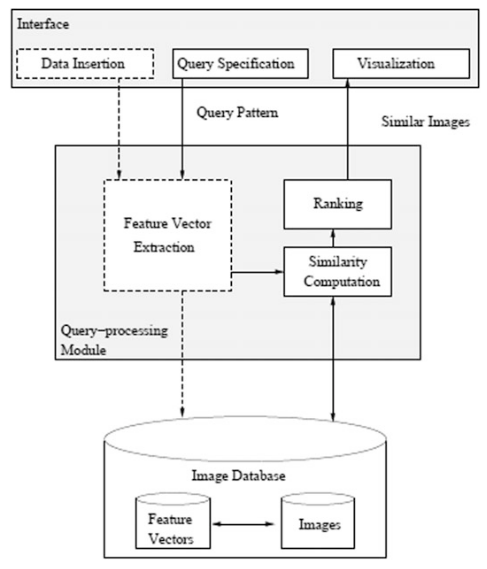
\includegraphics[width=0.55\textwidth]{content-based-esquema}
  \caption{Arquitectura de un sistema CBIR típico. \cite{content-based}}
  \label{fig:content-based-esquema}
\end{figure}

En las páginas 7-8 y 22-26 de \cite{report:39} se mencionan tres niveles de consultas en un CBIR siendo:

\begin{itemize}
\item Nivel 1: La recuperación de imágenes a través de características primitivas como pueden ser diferentes medidas de representación matemática de colores, texturas o formas. Un ejemplo sería un histograma de color que muestra la proporción de píxeles de cada color dentro de la imagen y la consulta sería encontrar imágenes con valores similares.
\item Nivel 2: Comprende la recuperación por características derivadas, también conocidas como lógicas, incluyendo un cierto grado de inferencia lógica sobre la identidad de los objetos representados en la imagen. Además puede ser dividido en:
\begin{itemize}
\item recuperación de objetos de un determinado tipo o categoría. Por ejemplo, ``encuentra imágenes de un autobús de dos pisos''.
\item recuperación de objetos individuales o personas. Por ejemplo, ``encuentra una imagen de la torre Eiffle''.
\end{itemize}
\item Nivel 3: Se trata de la recuperación por atributos abstractos, incluyendo una cantidad significativa de razonamiento de alto nivel sobre el propósito de los objetos o escenas representadas. Por ejemplo, ``encuentra imágenes de una multitud alegre''.
\end{itemize}

El objetivo de este proyecto es desarrollar una aplicación en java que represente un sistema CBIR que siga una arquitectura como la mostrada en \autoref{fig:content-based-esquema}. Este será capaz de extraer distintas características de una imagen y de comparar, o calcular la similitud, entre las imágenes de distintas formas para obtener distintas clasificaciones ordenadas que serán visualizadas en la aplicación. \\

Se podrán realizar consultas de nivel 1 a través de características de color y de nivel 2 utilizando segmentación semántica para la distinción de categorías con una red neuronal implementada en Python.

\chapter{Planificación y presupuesto.}
\chapter{Requisitos}
Antes de desarrollar la aplicación se debe comenzar con la exposición de los requisitos de datos, funcionales y no funcionales que esta requerirá para así poder tener en mente qué es lo que necesitamos, de qué es lo disponemos y cómo podremos trabajar de forma óptima para llegar al resultado deseado.\\

Teniendo en mente \autoref{fig:content-based-esquema}, sabemos que debemos de tener los siguientes requisitos de datos:\\
\begin{enumerate}
\item Representación de una imagen
\item Vector de características, en adelante descriptor, por cada característica que se quiera extraer o analizar.
\item Base de datos capaz de almacenar los descriptores correspondientes a cada una de las imágenes que estarán almacenadas en dicha base o fácilmente accesibles a través de la información almacenada en ella.
\item Representación de un descriptor genérico almacenado en la base de datos.
\item Concepto de clasificador utilizado para extraer las características.
\item Concepto de comparador para calcular la similitud entre las distintas características.
\end{enumerate}
Seguidamente, respecto a los requisitos funcionales debemos de considerar:\\
\begin{enumerate}
\item Abrir, guardar y cerrar una imagen.
\item Realización de consultas basadas en el contenido de una imagen.
\item Realización de consultas basadas en texto, siendo estas las categorías a las cuales pueden pertenecer nuestras imágenes.
\item Agrupación de categorías.
\item Extracción de descriptores de nivel 1.
\item Extracción de un descriptor de nivel 2.
\item Almacenaje de un conjunto de imágenes para poder ser comparadas.
\item Crear, modificar, guardar y abrir bases de datos.
\item Almacenaje de los descriptores correspondientes a dichas imágenes en una base de datos.
\item Enlace entre las imágenes y sus correspondientes descriptores para un fácil acceso.
\item Comparación entre descriptores.
\item Comparación utilizando múltiples descriptores de las propias imágenes.
\item Ordenación de imágenes resultantes de la consulta utilizando el resultado de la comparación entre descriptores.
\item Capacidad de visualizar las imágenes resultado de forma ordenada según la puntuación obtenida.
\item Capacidad de cambiar los comparadores utilizados sin que se vean afectados los descriptores utilizados.
\item Capacidad de crear nuevas bases de datos utilizando diferentes descriptores.
\item Capacidad de crear nuevas bases de datos utilizando múltiples descriptores.
\item Importar un clasificador a través de un fichero.
\end{enumerate}
Respecto a los requisitos no funcionales nos referimos a las características de funcionamiento que nos servirán para mantener la calidad de nuestro programa. Estos serán, principalmente: rendimiento, durabilidad, estabilidad, seguridad, eficiencia, compatibilidad, garantía e integración de datos.\\

Finalmente, se debe comentar que todo el proyecto deberá de poder ejecutarse en ordenadores que no dispongan de muchos recursos en unos tiempos razonables, al ser el material del que se dispone y siendo esta la prueba del funcionamiento en uno de los peores casos posibles.

\chapter{Análisis}
Comenzaremos analizando los requisitos mencionados en el capítulo anterior para poder enfrentarnos correctamente al diseño de nuestro sistema.\\

Para los requisitos de datos se considera el encapsular apropiadamente cada uno de estos en una clase propia que sirva como una correcta representación de cada uno de los conceptos. En particular, si consideramos las especificaciones planteadas en los requisitos funcionales, se hace evidente la necesidad de la utilización de herencia para un correcto diseño del software al haber conceptos genéricos que más adelante se dividen teniendo diferentes especificaciones.\\

Además, es necesario desarrollar una aplicación de escritorio que haga mucho más intuitivo la utilización de cada uno de los elementos a implementar. Así, alguien sin conocimientos de programación, pero con interés o una cantidad relativa de estudios en la materia, podría utilizarla cómodamente.\\

Teniendo también en cuenta que sería ideal que la aplicación fuese multiplataforma y la existencia de la \emph{Java Multimedia Retrieval (JMR)} \cite{JMR}, librería desarrollada por Jesús Chamorro Martínez que resuelve de forma genérica gran parte de las funcionalidades solicitadas, se ha decidido utilizar Java como lenguaje de programación.\\

Sin embargo, se debe de tener en cuenta que este proyecto ha sido planteado bajo la premisa de la utilización de aprendizaje profundo. Este será utilizado para la extracción de características de nivel 2, mediante la utilización de una red neuronal convolucionada \autoref{ch:cnn} que realizará una segmentación semántica para obtener diversas categorías así como los píxeles concretos de cada imagen que pertenecerán a cada categoría \cite{ch:fast-attention}.\\

Si bien existen bibliotecas para el aprendizaje profundo en Java, estas no están tan desarrolladas como podrían estarlo en otros lenguajes de programación como Python. Por ello, se utilizará Python 3 para la creación, el entrenamiento y la carga de los modelos que se lleguen a probar a lo largo del proyecto.\\

Esto plantea la cuestión de cómo resolver la comunicación entre los distintos lenguajes, que será resulta mediante la utilización de una conexión TCP.\\
\chapter{Diseño}

Como se mencionó en el capítulo anterior, la aplicación será diseñada en dos partes conectadas por una conexión TCP. Comenzaremos mencionando las librerías utilizadas para cada una de las partes, prosiguiendo con mostrar una serie de diagramas que mostrarán la estructura interna utilizará nuestra aplicación haciendo uso del material disponible.

\section{Librerías utilizadas}

Comenzaremos mencionando las librerías utilizadas para la creación, entrenamiento y carga de la red neuronal. Principalmente se ha utilizado:
\begin{enumerate}
\item Tensorflow \cite{tensorflow2015-whitepaper}:  se trata de una plataforma de código abierto de extremo a extremo para el aprendizaje automático. Posee una API para diversos lenguajes de programación como son Javascript y Python además de estar disponible tanto para ordenadores como para dispositivos móviles, en este caso bajo su versión Tensorflow Lite. Como extra, permite utilizar varias CPUs o GPUs, con la consecuente posibilidad de aceleración GPU, y ofrece soporte experimental para \emph{Cloud TPUs} en Keras y Google Colab. En particular se utilizará Tensorflow 2.0 que es compatible con Python 3.5 a 3.8.
\item Keras \cite{chollet2015keras} : es una API construida sobre TensorFlow 2.0 que, según su propia página web, ``está diseñada para seres humanos, no para máquinas''. Está optimizada para GPU, CPU y TPU.Fue concebida para actuar como una interfaz en lugar de un framework de machine learning standalone por lo que ofrece un conjunto de abstracciones más intuitivas y de alto nivel, haciendo más sencillo el desarrollo de modelos de aprendizaje profundo.
\item Classification models Zoo - Keras \cite{classification_models}: se trata de un conjunto de clasificadores entrenados en el conjunto de datos ImageNet \cite{imagenet_cvpr09}. De esta forma podremos obtener clasificadores que no están disponibles ni en Keras ni en TensorFlow, en particular ResNet18 \cite{DBLP:journals/corr/HeZRS15}.
\item Imgaug \cite{imgaug} es una biblioteca para el aumento de imágenes en los experimentos de aprendizaje automático. Soporta un gran rango de técnicas de aumento de datos, permite combinarlas fácilmente y ejecutarlas de forma aleatoria en múltiples núcleos CPU.
\end{enumerate}

Para el tratamiento de los datos resultantes de la red neuronal con el fin de adaptarlos para utilizarlos en la aplicación, se ha utilizado el ecosistema basado en Python SciPy, principalmente las librerías:
\begin{enumerate}
\item SciPy \cite{2020SciPy-NMeth} librería fundamental para el cálculo científico.
\item NumPy \cite{2020NumPy-Array} paquete de vectores n-dimensionales.
\item Pandas \cite{reback2020pandas} \cite{mckinney-proc-scipy-2010} estructura de datos y análisis.
\item Matplotlib \cite{Hunter:2007} trazado completo en 2D.
\end{enumerate}
Además, se ha utilizado scikit-image \cite{scikit-image} (o skimage) que es una colección de algoritmos para procesamiento de imágenes y la visión por computador.\\

Como se mencionó en el capítulo anterior, para como esqueleto genérico del sistema CBIR se utilizará la biblioteca \emph{Java Multimedia Retrieval (JMR)} \cite{JMR} sobre la cual desarrollaremos en más detalle los elementos que utilizaremos. En particular, estaremos utilizando una versión actualizada por Miriam Mengíbar Rodríguez para su trabajo de fin de master \cite{TFM}.\\

\begin{figure}[htpb]
  \centering
  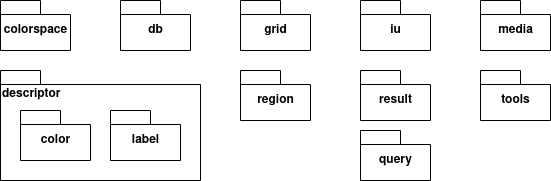
\includegraphics[width=0.9\textwidth]{jmrpackage}
  \caption{Diagrama representante de algunos de los paquetes de la JMR. \cite{JMR}}
  \label{fig:jmrpackage}
\end{figure}

De los paquetes mostrados, concretamente se utilizarán:
\begin{itemize}
\item \emph{db} : Paquete que simula una base de datos. Posee su propio elemento creado a partir de los datos de entrada y de los descriptores, compatibles con la comparación con las consultas y con una cómoda recuperación de los datos originales.
\item \emph{descriptor} : Paquete que engloba los elementos necesarios para una correcta representación de un descriptor o vector de características, como es el caso de la interfaz \emph{Comparator} o la interfaz \emph{MediaDescriptor}. Posee dos subpaquetes:
\begin{itemize}
\item \emph{descriptor.color} : Paquete que implementa descriptores de colores de acuerdo al estándar MPEG7 \cite{MPPEG7}.
\item \emph{descriptor.label} : Paquete que implementa un descriptor por etiquetas genérico así como definir las interfaces necesarias para la clasificación de las etiquetas.
\end{itemize}
\item \emph{region} : Paquete diseñado para la representación de una región contenida en una imagen. Si bien este paquete no se ha utilizado directamente, servirá como inspiración para la definición de la clase \emph{MultiRegion} que se verá más adelante.
\end{itemize}

Además, también se utilizarán las clases \emph{LabelGroup} y \emph{TCPClient}, siendo esta última a través de la cual se consigue la conexión TCP con el módulo de python, ambas implementas por Miriam en su trabajo de fin de master \cite{TFM}.

\newpage
\section{Descriptores}
A la hora de diseñar los descriptores, debemos de tener especial atención en no diseñar nada de lo que ya dispongamos. Por ello, no será necesario el diseño de descriptores de nivel 1 de tipo color, puesto que estos ya están diseñados e implementados a través de los paquetes \emph{descriptor} y \emph{descriptor.color} de la JMR \cite{JMR}.\\

El principal trabajo será el diseño e implementación de un descriptor de nivel 2 con su respectivo comparador. En particular, se ha diseñado el descriptor \emph{RegionLabelDescriptor} que, dada una imagen, describirá cada una de las categorías pertenecientes a dicha imagen así como los píxeles concretos que pertenecerán a cada una de estas categorías. De esta forma, no sólo conoceremos qué etiquetas o categorías estarán presentes en la propia imagen sino que además la localización a nivel de píxel de cada una de estas categorías.\\

\begin{figure}[htpb]
  \centering
  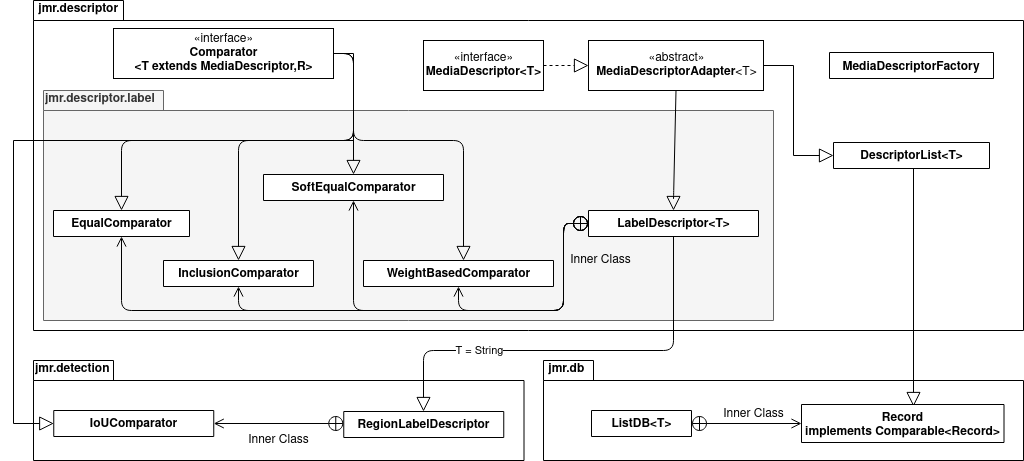
\includegraphics[width=1.1\textwidth]{DescriptorsAndComparators}
  \caption{Diagrama de herencia y clases internas para los descriptores y comparadores de etiquetas. \cite{JMR}}
  \label{fig:DescriptorsAndComparators}
\end{figure}

Para la extracción de estas características para la creación de este descriptor, se ha definido un clasificador llamado \emph{AttentionClassifier} que recibirá la url de la imagen cuyas características se desean extraer y, a través del uso de la clase \emph{TCPClient}, se conectará con un servidor de python llamado \emph{server.py} que segmentará semánticamente la imagen. Con esta información, almacenada en un objeto de la clase \emph{RegionClassification}, se construirá correctamente un objeto \emph{RegionLabelDescriptor} que podrá ser comparado utilizando los comparadores internos de su clase madre \emph{LabelDescriptor} y el comparador \emph{IoUComparator} que se definirá y creará para este descriptor concreto.\\

\begin{figure}[htpb]
  \centering
  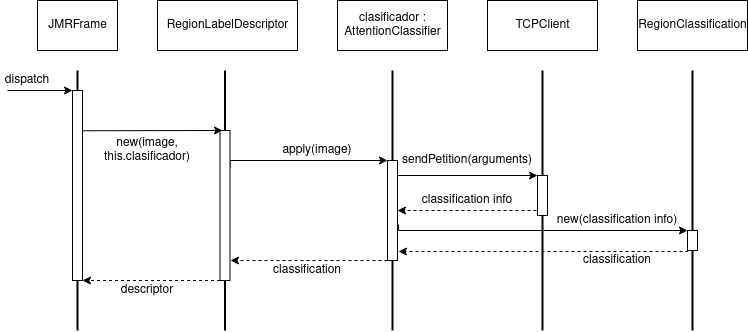
\includegraphics[width=1.1\textwidth]{DiagramaSecuencia}
  \caption{Diagrama de secuencia que muestra la creación de un descriptor del tipo \emph{RegionLabelDescriptor}}
  \label{fig:DiagramaSecuencia}
\end{figure}

Un detalle importante a tener en cuenta, se trata de que, mientras que en los descriptores de color se definen con \emph{T=BufferedImage}, para el nuevo descriptor que estaremos creando se utilizará \emph{T=String} siendo este \emph{string} la dirección donde esta almacenada en nuestro dispositivo la imagen representante. Se ha elegido este método para facilitar la conexión TCP, así como su velocidad, pero tendremos la desventaja de que no podremos crear una base de datos que contemple tanto descriptores de color como descriptores de regiones al estar trabajando sobre tipos distintos.\\

Resumiendo, se deberán de implementar las clases \emph{RegionLabelDescriptor}, \emph{AttentionClassifier} y \emph{RegionClassification} para tener la funcionalidad del descriptor deseado. Además, también se implementará la clase \emph{IoUComparator} para añadir una nueva opción de comparación entre descriptores.\\

En la sección de implementación, se describirá el funcionamiento de \emph{IoUComparator} así como el funcionamiento y utilidad de otras clases desarrolladas para facilitar la comunicación con \emph{JMRFrame}, en particular se tratará de la clase \emph{MultiRegion} y de clases que tendrán la funcionalidad de renderizar la información de los cuadros combinados a implementar en la interfaz de usuario.

\chapter{Implementación}
Para la implementación con el lenguaje Java se ha utilizado el entorno de desarrollo \emph{Apache Netbeans IDE 12.1}, sobre todo teniendo en mente el desarrollo de la interfaz gráfica que se ve sumamente facilitado gracias a las herramientas de la que dispone esta interfaz de desarrollo. Mientras que para el código en python y la propia memoria se ha utilizado el editor \emph{Atom} que permite una comunicación interactiva con el repositorio de GitHub utilizado para este proyecto \cite{GitHub} en el cual se pondrá encontrar todo el código desarrollado.\\

Además, se podrán encontrar en dicho repositorio algunos de los múltiples entrenamientos de redes neuronales realizados así como cuadernillos de \emph{Jupyter Notebook} que mostrarán los diversos detalles de estos. Así, se podrá ver de forma interactiva los detalles analizados, en caso de ser de interés, sin necesidad de extender más de lo necesario esta memoria.
\section{Comparadores}

Antes de proceder a explicar la implementación de la clase \emph{IoUComparator} es necesario que se haga una pequeña pausa para comprender el funcionamiento de los comparadores de los ya existentes, en particular los pertenecientes a \emph{LabelDescriptor} para asegurarnos tener una buena compatibilidad con ellos y poder comprender mejor la futura implementación de \emph{IoUComparator}.\\

Dados dos descriptores, la imagen de la función de comparación entre ambos será $[0,+\infty]$, donde el resultado $0$ indicará que bajo esta comparación son iguales y cualquier otro valor significará que son distintos indicando una medida de la diferencia de relativa a esos dos descriptores bajo dicha comparación. En particular, el valor $+\infty$ representará la máxima diferencia posible, también interpretable como incomparables.\\

Sabiendo que un descriptor de tipo \emph{LabelDescriptor} posee un vector de etiquetas de tipo \emph{string}, se dirá que un \emph{LabelDescriptor} $t$ está incluido en otro \emph{LabelDescriptor} $u$ si cada etiqueta perteneciente al vector de etiquetas de $t$ esta incluida en el vector de etiquetas de $u$. En particular, si existen etiquetas repetidas en $t$ bastará con que estas aparezcan una única vez en $u$ para que se siga considerando como verdadera la relación $t \subset u$, o $t$ incluido en $u$.\\

Dicho esto, podemos explicar el comportamiento de los descriptores sin pesos de \emph{LabelDescriptor}. Sean $t$ y $u$ dos \emph{LabelDescriptor}, el comparador
\begin{itemize}
\item \emph{InclusionComparator} devolverá la igualdad, es decir, el valor $0$ si $t\subset u$. Se retornará $+\infty$ si no se cumple la relación.
\item \emph{SoftEqualComparator} devolverá la igualdad, es decir, el valor $0$ si $t\subset u$ o $u\subset t$. Se retornará $+\infty$ si no se cumple ninguna relación.
\item \emph{EqualComparator} devolverá la igualdad, es decir, el valor $0$ si $t \subset u $, $u \subset t$ y tanto $t$ como $u$ poseen la misma cantidad de etiquetas. Se retornará $+\infty$ si no se cumplen ambas relaciones.
\end{itemize}

Por otro lado, si se le añade un valor de pesos no nulo a cada una de las etiquetas de un \emph{LabelDescriptor}, por defecto, se utiliza el \emph{WeightBasedComparator} que permite elegir entre la utilización de comparación con igualdad o inclusión de etiquetas, además de calcular el valor absoluto de la diferencia de pesos de las etiquetas. Se permite elegir entre devolver el máximo, mínimo, media aritmética o media euclídea de los resultados de cada valor absoluto de la diferencia de las etiquetas como valor real, teniendo en cuenta que se devolverá, además, $+\infty$ en caso de que este sea el valor devuelto por la operación de igualdad o inclusión seleccionada.\\

Una vez explicado esto, se procederá a realizar las explicación de la implementación del \emph{IoUComparator} que ha sido desarrollado para este proyecto.\\

Comenzando, realiza una comparación por etiquetas utilizando \emph{EqualComparator} o \emph{InclusionComparator} según se desee, devolviendo $+\infty$ en caso de que este sea el resultado de esta primera comparación.\\

Si se obtiene un valor distinto, se procede a unificar temporalmente las categorías duplicadas de forma que las siguientes operaciones se realicen de forma independiente para cada categoría distinta. Seguidamente, para cada categoría se calcula la cantidad de píxeles que pertenecen a la intersección de esta categoría para el \emph{RegionLabelDescriptor} $t$ y el \emph{RegionLabelDescriptor} $u$, de la misma forma se contabiliza para la unión y se divide el valor de la intersección entre la unión.\\

Con esta operación, obtendremos tenderemos al valor $0$ cuantos menos píxeles coincidan en ambas imágenes y obtendremos el valor $1$ si todos los píxeles de la categoría seleccionada coinciden. Sin embargo, estos valores no comparten el mismo criterio que compartían los comparadores de la clase madre, por lo que aplicaremos una transformación no lineal para seguir el mismo criterio. En concreto, se hará:

$$\frac{1}{IoU}-1,$$

que devolverá $0$ si ambas comparten los mismos píxeles en la categoría y tenderá a $+\infty$ cuantos menos píxeles coincidan.\\

Finalmente, de forma similar a como sucedía en \emph{WeightBasedComparator}, se permite elegir entre el máximo, mínimo, media aritmética o media euclídea para obtener el resultado final a partir de los resultados parciales correspondientes a cada categoría, siendo este el valor devuelto para la comparación de los dos descriptores.\\

FIXME: Añadir un diagramaita que simplifique la explicación
